\thesolution{Lista Semplicemente Collegata}%{LinkedList}
Di seguito si riporta il file \cod{Lista.h} contenente la dichiarazione della classe \cod{Lista}, oltre che le definizioni dei tipi \cod{Record} e \cod{TElem} funzionali all'uso della classe. La dichiarazione del tipo \cod{Record}, che rappresenta la generica cella della lista, rispetta il principio dell'\emph{information hiding}; tale tipo infatti � esclusivamente dichiarato, e sar� definito solo successivamente nel file \cod{Lista.cpp}. La sua struttura interna risulta pertanto inaccessibile agli utenti della classe.

\enablelstnum
\inputmodule{Lista.h}{Esercizi/LinkedList/Lista.h}

Le prime due righe del file appena mostrato, insieme con l'ultima, impediscono che il file \cod{Lista.h} possa essere processato dal pre-compilatore pi� di una volta all'atto della compilazione di un file sorgente. Ci� accade nell'eventualit� che, nel grafo delle inclusioni che va a formarsi all'atto della compilazione di un file \cod{.cpp}, il file \cod{Lista.h} risulti incluso da pi� di un file. Dal momento che l'header file \cod{Lista.h} contiene esclusivamente dichiarazioni (e non definizioni), una sua eventuale inclusione multipla sarebbe ininfluente ai fini della compilazione.

Si noti inoltre come l'operatore di assegnazione della lista riportato alla riga 13 sia dichiarato tra i metodi privati della classe, nonostante non verr� successivamente definito nel relativo file \cod{.cpp}. Tale dichiarazione � esclusivamente finalizzata ad impedire che tale metodo possa essere invocato dagli utenti della classe \cod{Lista}. Se ci� accadesse, infatti, verrebbe invocata l'implementazione dell'operatore di assegnazione automaticamente sintetizzata dal compilatore e consistente in una copia bit a bit dei membri della classe, verosimilmente scorretta ai fini di un utilizzo reale della struttura (\seename~\cite{EffC++}).

\inputmodule{Lista.cpp}{Esercizi/LinkedList/Lista.cpp}
\inputmodule{main.cpp}{Esercizi/LinkedList/main.cpp}

\subsubsection*{Implementazione alternativa del metodo \cod{Lista::Elimina()}}

\`E possibile realizzare un'implementazione alternativa del metodo \cod{Elimina()}, ancora pi� sintetica di quella appena mostrata. Tale variante, a differenza dell'implementazione precedente, non discrimina il caso in cui l'elemento da eliminare sia posizionato in testa alla struttura, ma tratta i due casi in maniera omogenea. Per ottenere questo, � sufficiente utilizzare un puntatore a \cod{PRec} (puntatore a puntatore --- vedi \figurename~\ref{fig:PuntPunt}).

\begin{figure}
  \center
	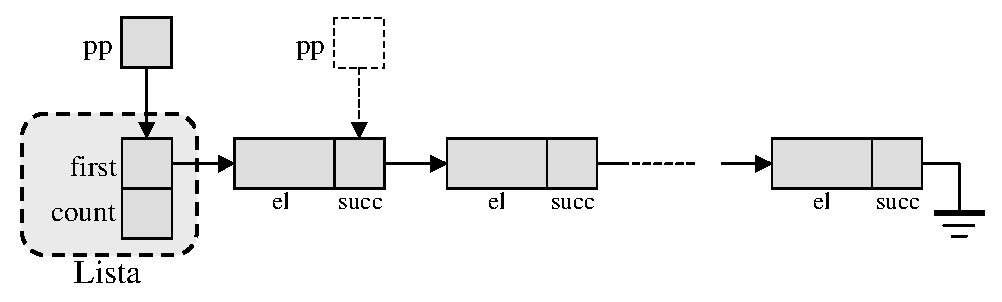
\includegraphics[width=.8\textwidth]{Esercizi/LinkedList/PuntPunt.eps}
	\caption{Un puntatore ``scorre'' la lista puntando ai puntatori contenuti in essa.}
	\label{fig:PuntPunt}
\end{figure}

Inizialmente il puntatore \cod{pp} definito del tipo \cod{PRec*} punta alla locazione \cod{first}, membro privato della lista (linea continua). Nella (eventuale) seconda iterazione, esso passa a puntare alla locazione \cod{succ} dell'elemento di testa (linea tratteggiata). In tale passaggio la compatibilit� di tipo � rispettata, essendo sia \cod{first} che il campo \cod{succ} del tipo \cod{Record} dichiarati di tipo \cod{PRec}.

\bigskip
\inputprogram{Esercizi/LinkedList/EliminaSpare.cpp}